
% Default to the notebook output style

    


% Inherit from the specified cell style.




    
\documentclass[11pt]{article}

    
    
    \usepackage[T1]{fontenc}
    % Nicer default font (+ math font) than Computer Modern for most use cases
    \usepackage{mathpazo}

    % Basic figure setup, for now with no caption control since it's done
    % automatically by Pandoc (which extracts ![](path) syntax from Markdown).
    \usepackage{graphicx}
    % We will generate all images so they have a width \maxwidth. This means
    % that they will get their normal width if they fit onto the page, but
    % are scaled down if they would overflow the margins.
    \makeatletter
    \def\maxwidth{\ifdim\Gin@nat@width>\linewidth\linewidth
    \else\Gin@nat@width\fi}
    \makeatother
    \let\Oldincludegraphics\includegraphics
    % Set max figure width to be 80% of text width, for now hardcoded.
    \renewcommand{\includegraphics}[1]{\Oldincludegraphics[width=.8\maxwidth]{#1}}
    % Ensure that by default, figures have no caption (until we provide a
    % proper Figure object with a Caption API and a way to capture that
    % in the conversion process - todo).
    \usepackage{caption}
    \DeclareCaptionLabelFormat{nolabel}{}
    \captionsetup{labelformat=nolabel}

    \usepackage{adjustbox} % Used to constrain images to a maximum size 
    \usepackage{xcolor} % Allow colors to be defined
    \usepackage{enumerate} % Needed for markdown enumerations to work
    \usepackage{geometry} % Used to adjust the document margins
    \usepackage{amsmath} % Equations
    \usepackage{amssymb} % Equations
    \usepackage{textcomp} % defines textquotesingle
    % Hack from http://tex.stackexchange.com/a/47451/13684:
    \AtBeginDocument{%
        \def\PYZsq{\textquotesingle}% Upright quotes in Pygmentized code
    }
    \usepackage{upquote} % Upright quotes for verbatim code
    \usepackage{eurosym} % defines \euro
    \usepackage[mathletters]{ucs} % Extended unicode (utf-8) support
    \usepackage[utf8x]{inputenc} % Allow utf-8 characters in the tex document
    \usepackage{fancyvrb} % verbatim replacement that allows latex
    \usepackage{grffile} % extends the file name processing of package graphics 
                         % to support a larger range 
    % The hyperref package gives us a pdf with properly built
    % internal navigation ('pdf bookmarks' for the table of contents,
    % internal cross-reference links, web links for URLs, etc.)
    \usepackage{hyperref}
    \usepackage{longtable} % longtable support required by pandoc >1.10
    \usepackage{booktabs}  % table support for pandoc > 1.12.2
    \usepackage[inline]{enumitem} % IRkernel/repr support (it uses the enumerate* environment)
    \usepackage[normalem]{ulem} % ulem is needed to support strikethroughs (\sout)
                                % normalem makes italics be italics, not underlines
    

    
    
    % Colors for the hyperref package
    \definecolor{urlcolor}{rgb}{0,.145,.698}
    \definecolor{linkcolor}{rgb}{.71,0.21,0.01}
    \definecolor{citecolor}{rgb}{.12,.54,.11}

    % ANSI colors
    \definecolor{ansi-black}{HTML}{3E424D}
    \definecolor{ansi-black-intense}{HTML}{282C36}
    \definecolor{ansi-red}{HTML}{E75C58}
    \definecolor{ansi-red-intense}{HTML}{B22B31}
    \definecolor{ansi-green}{HTML}{00A250}
    \definecolor{ansi-green-intense}{HTML}{007427}
    \definecolor{ansi-yellow}{HTML}{DDB62B}
    \definecolor{ansi-yellow-intense}{HTML}{B27D12}
    \definecolor{ansi-blue}{HTML}{208FFB}
    \definecolor{ansi-blue-intense}{HTML}{0065CA}
    \definecolor{ansi-magenta}{HTML}{D160C4}
    \definecolor{ansi-magenta-intense}{HTML}{A03196}
    \definecolor{ansi-cyan}{HTML}{60C6C8}
    \definecolor{ansi-cyan-intense}{HTML}{258F8F}
    \definecolor{ansi-white}{HTML}{C5C1B4}
    \definecolor{ansi-white-intense}{HTML}{A1A6B2}

    % commands and environments needed by pandoc snippets
    % extracted from the output of `pandoc -s`
    \providecommand{\tightlist}{%
      \setlength{\itemsep}{0pt}\setlength{\parskip}{0pt}}
    \DefineVerbatimEnvironment{Highlighting}{Verbatim}{commandchars=\\\{\}}
    % Add ',fontsize=\small' for more characters per line
    \newenvironment{Shaded}{}{}
    \newcommand{\KeywordTok}[1]{\textcolor[rgb]{0.00,0.44,0.13}{\textbf{{#1}}}}
    \newcommand{\DataTypeTok}[1]{\textcolor[rgb]{0.56,0.13,0.00}{{#1}}}
    \newcommand{\DecValTok}[1]{\textcolor[rgb]{0.25,0.63,0.44}{{#1}}}
    \newcommand{\BaseNTok}[1]{\textcolor[rgb]{0.25,0.63,0.44}{{#1}}}
    \newcommand{\FloatTok}[1]{\textcolor[rgb]{0.25,0.63,0.44}{{#1}}}
    \newcommand{\CharTok}[1]{\textcolor[rgb]{0.25,0.44,0.63}{{#1}}}
    \newcommand{\StringTok}[1]{\textcolor[rgb]{0.25,0.44,0.63}{{#1}}}
    \newcommand{\CommentTok}[1]{\textcolor[rgb]{0.38,0.63,0.69}{\textit{{#1}}}}
    \newcommand{\OtherTok}[1]{\textcolor[rgb]{0.00,0.44,0.13}{{#1}}}
    \newcommand{\AlertTok}[1]{\textcolor[rgb]{1.00,0.00,0.00}{\textbf{{#1}}}}
    \newcommand{\FunctionTok}[1]{\textcolor[rgb]{0.02,0.16,0.49}{{#1}}}
    \newcommand{\RegionMarkerTok}[1]{{#1}}
    \newcommand{\ErrorTok}[1]{\textcolor[rgb]{1.00,0.00,0.00}{\textbf{{#1}}}}
    \newcommand{\NormalTok}[1]{{#1}}
    
    % Additional commands for more recent versions of Pandoc
    \newcommand{\ConstantTok}[1]{\textcolor[rgb]{0.53,0.00,0.00}{{#1}}}
    \newcommand{\SpecialCharTok}[1]{\textcolor[rgb]{0.25,0.44,0.63}{{#1}}}
    \newcommand{\VerbatimStringTok}[1]{\textcolor[rgb]{0.25,0.44,0.63}{{#1}}}
    \newcommand{\SpecialStringTok}[1]{\textcolor[rgb]{0.73,0.40,0.53}{{#1}}}
    \newcommand{\ImportTok}[1]{{#1}}
    \newcommand{\DocumentationTok}[1]{\textcolor[rgb]{0.73,0.13,0.13}{\textit{{#1}}}}
    \newcommand{\AnnotationTok}[1]{\textcolor[rgb]{0.38,0.63,0.69}{\textbf{\textit{{#1}}}}}
    \newcommand{\CommentVarTok}[1]{\textcolor[rgb]{0.38,0.63,0.69}{\textbf{\textit{{#1}}}}}
    \newcommand{\VariableTok}[1]{\textcolor[rgb]{0.10,0.09,0.49}{{#1}}}
    \newcommand{\ControlFlowTok}[1]{\textcolor[rgb]{0.00,0.44,0.13}{\textbf{{#1}}}}
    \newcommand{\OperatorTok}[1]{\textcolor[rgb]{0.40,0.40,0.40}{{#1}}}
    \newcommand{\BuiltInTok}[1]{{#1}}
    \newcommand{\ExtensionTok}[1]{{#1}}
    \newcommand{\PreprocessorTok}[1]{\textcolor[rgb]{0.74,0.48,0.00}{{#1}}}
    \newcommand{\AttributeTok}[1]{\textcolor[rgb]{0.49,0.56,0.16}{{#1}}}
    \newcommand{\InformationTok}[1]{\textcolor[rgb]{0.38,0.63,0.69}{\textbf{\textit{{#1}}}}}
    \newcommand{\WarningTok}[1]{\textcolor[rgb]{0.38,0.63,0.69}{\textbf{\textit{{#1}}}}}
    
    
    % Define a nice break command that doesn't care if a line doesn't already
    % exist.
    \def\br{\hspace*{\fill} \\* }
    % Math Jax compatability definitions
    \def\gt{>}
    \def\lt{<}
    % Document parameters
    \title{Presentation}
    
    
    

    % Pygments definitions
    
\makeatletter
\def\PY@reset{\let\PY@it=\relax \let\PY@bf=\relax%
    \let\PY@ul=\relax \let\PY@tc=\relax%
    \let\PY@bc=\relax \let\PY@ff=\relax}
\def\PY@tok#1{\csname PY@tok@#1\endcsname}
\def\PY@toks#1+{\ifx\relax#1\empty\else%
    \PY@tok{#1}\expandafter\PY@toks\fi}
\def\PY@do#1{\PY@bc{\PY@tc{\PY@ul{%
    \PY@it{\PY@bf{\PY@ff{#1}}}}}}}
\def\PY#1#2{\PY@reset\PY@toks#1+\relax+\PY@do{#2}}

\expandafter\def\csname PY@tok@w\endcsname{\def\PY@tc##1{\textcolor[rgb]{0.73,0.73,0.73}{##1}}}
\expandafter\def\csname PY@tok@c\endcsname{\let\PY@it=\textit\def\PY@tc##1{\textcolor[rgb]{0.25,0.50,0.50}{##1}}}
\expandafter\def\csname PY@tok@cp\endcsname{\def\PY@tc##1{\textcolor[rgb]{0.74,0.48,0.00}{##1}}}
\expandafter\def\csname PY@tok@k\endcsname{\let\PY@bf=\textbf\def\PY@tc##1{\textcolor[rgb]{0.00,0.50,0.00}{##1}}}
\expandafter\def\csname PY@tok@kp\endcsname{\def\PY@tc##1{\textcolor[rgb]{0.00,0.50,0.00}{##1}}}
\expandafter\def\csname PY@tok@kt\endcsname{\def\PY@tc##1{\textcolor[rgb]{0.69,0.00,0.25}{##1}}}
\expandafter\def\csname PY@tok@o\endcsname{\def\PY@tc##1{\textcolor[rgb]{0.40,0.40,0.40}{##1}}}
\expandafter\def\csname PY@tok@ow\endcsname{\let\PY@bf=\textbf\def\PY@tc##1{\textcolor[rgb]{0.67,0.13,1.00}{##1}}}
\expandafter\def\csname PY@tok@nb\endcsname{\def\PY@tc##1{\textcolor[rgb]{0.00,0.50,0.00}{##1}}}
\expandafter\def\csname PY@tok@nf\endcsname{\def\PY@tc##1{\textcolor[rgb]{0.00,0.00,1.00}{##1}}}
\expandafter\def\csname PY@tok@nc\endcsname{\let\PY@bf=\textbf\def\PY@tc##1{\textcolor[rgb]{0.00,0.00,1.00}{##1}}}
\expandafter\def\csname PY@tok@nn\endcsname{\let\PY@bf=\textbf\def\PY@tc##1{\textcolor[rgb]{0.00,0.00,1.00}{##1}}}
\expandafter\def\csname PY@tok@ne\endcsname{\let\PY@bf=\textbf\def\PY@tc##1{\textcolor[rgb]{0.82,0.25,0.23}{##1}}}
\expandafter\def\csname PY@tok@nv\endcsname{\def\PY@tc##1{\textcolor[rgb]{0.10,0.09,0.49}{##1}}}
\expandafter\def\csname PY@tok@no\endcsname{\def\PY@tc##1{\textcolor[rgb]{0.53,0.00,0.00}{##1}}}
\expandafter\def\csname PY@tok@nl\endcsname{\def\PY@tc##1{\textcolor[rgb]{0.63,0.63,0.00}{##1}}}
\expandafter\def\csname PY@tok@ni\endcsname{\let\PY@bf=\textbf\def\PY@tc##1{\textcolor[rgb]{0.60,0.60,0.60}{##1}}}
\expandafter\def\csname PY@tok@na\endcsname{\def\PY@tc##1{\textcolor[rgb]{0.49,0.56,0.16}{##1}}}
\expandafter\def\csname PY@tok@nt\endcsname{\let\PY@bf=\textbf\def\PY@tc##1{\textcolor[rgb]{0.00,0.50,0.00}{##1}}}
\expandafter\def\csname PY@tok@nd\endcsname{\def\PY@tc##1{\textcolor[rgb]{0.67,0.13,1.00}{##1}}}
\expandafter\def\csname PY@tok@s\endcsname{\def\PY@tc##1{\textcolor[rgb]{0.73,0.13,0.13}{##1}}}
\expandafter\def\csname PY@tok@sd\endcsname{\let\PY@it=\textit\def\PY@tc##1{\textcolor[rgb]{0.73,0.13,0.13}{##1}}}
\expandafter\def\csname PY@tok@si\endcsname{\let\PY@bf=\textbf\def\PY@tc##1{\textcolor[rgb]{0.73,0.40,0.53}{##1}}}
\expandafter\def\csname PY@tok@se\endcsname{\let\PY@bf=\textbf\def\PY@tc##1{\textcolor[rgb]{0.73,0.40,0.13}{##1}}}
\expandafter\def\csname PY@tok@sr\endcsname{\def\PY@tc##1{\textcolor[rgb]{0.73,0.40,0.53}{##1}}}
\expandafter\def\csname PY@tok@ss\endcsname{\def\PY@tc##1{\textcolor[rgb]{0.10,0.09,0.49}{##1}}}
\expandafter\def\csname PY@tok@sx\endcsname{\def\PY@tc##1{\textcolor[rgb]{0.00,0.50,0.00}{##1}}}
\expandafter\def\csname PY@tok@m\endcsname{\def\PY@tc##1{\textcolor[rgb]{0.40,0.40,0.40}{##1}}}
\expandafter\def\csname PY@tok@gh\endcsname{\let\PY@bf=\textbf\def\PY@tc##1{\textcolor[rgb]{0.00,0.00,0.50}{##1}}}
\expandafter\def\csname PY@tok@gu\endcsname{\let\PY@bf=\textbf\def\PY@tc##1{\textcolor[rgb]{0.50,0.00,0.50}{##1}}}
\expandafter\def\csname PY@tok@gd\endcsname{\def\PY@tc##1{\textcolor[rgb]{0.63,0.00,0.00}{##1}}}
\expandafter\def\csname PY@tok@gi\endcsname{\def\PY@tc##1{\textcolor[rgb]{0.00,0.63,0.00}{##1}}}
\expandafter\def\csname PY@tok@gr\endcsname{\def\PY@tc##1{\textcolor[rgb]{1.00,0.00,0.00}{##1}}}
\expandafter\def\csname PY@tok@ge\endcsname{\let\PY@it=\textit}
\expandafter\def\csname PY@tok@gs\endcsname{\let\PY@bf=\textbf}
\expandafter\def\csname PY@tok@gp\endcsname{\let\PY@bf=\textbf\def\PY@tc##1{\textcolor[rgb]{0.00,0.00,0.50}{##1}}}
\expandafter\def\csname PY@tok@go\endcsname{\def\PY@tc##1{\textcolor[rgb]{0.53,0.53,0.53}{##1}}}
\expandafter\def\csname PY@tok@gt\endcsname{\def\PY@tc##1{\textcolor[rgb]{0.00,0.27,0.87}{##1}}}
\expandafter\def\csname PY@tok@err\endcsname{\def\PY@bc##1{\setlength{\fboxsep}{0pt}\fcolorbox[rgb]{1.00,0.00,0.00}{1,1,1}{\strut ##1}}}
\expandafter\def\csname PY@tok@kc\endcsname{\let\PY@bf=\textbf\def\PY@tc##1{\textcolor[rgb]{0.00,0.50,0.00}{##1}}}
\expandafter\def\csname PY@tok@kd\endcsname{\let\PY@bf=\textbf\def\PY@tc##1{\textcolor[rgb]{0.00,0.50,0.00}{##1}}}
\expandafter\def\csname PY@tok@kn\endcsname{\let\PY@bf=\textbf\def\PY@tc##1{\textcolor[rgb]{0.00,0.50,0.00}{##1}}}
\expandafter\def\csname PY@tok@kr\endcsname{\let\PY@bf=\textbf\def\PY@tc##1{\textcolor[rgb]{0.00,0.50,0.00}{##1}}}
\expandafter\def\csname PY@tok@bp\endcsname{\def\PY@tc##1{\textcolor[rgb]{0.00,0.50,0.00}{##1}}}
\expandafter\def\csname PY@tok@fm\endcsname{\def\PY@tc##1{\textcolor[rgb]{0.00,0.00,1.00}{##1}}}
\expandafter\def\csname PY@tok@vc\endcsname{\def\PY@tc##1{\textcolor[rgb]{0.10,0.09,0.49}{##1}}}
\expandafter\def\csname PY@tok@vg\endcsname{\def\PY@tc##1{\textcolor[rgb]{0.10,0.09,0.49}{##1}}}
\expandafter\def\csname PY@tok@vi\endcsname{\def\PY@tc##1{\textcolor[rgb]{0.10,0.09,0.49}{##1}}}
\expandafter\def\csname PY@tok@vm\endcsname{\def\PY@tc##1{\textcolor[rgb]{0.10,0.09,0.49}{##1}}}
\expandafter\def\csname PY@tok@sa\endcsname{\def\PY@tc##1{\textcolor[rgb]{0.73,0.13,0.13}{##1}}}
\expandafter\def\csname PY@tok@sb\endcsname{\def\PY@tc##1{\textcolor[rgb]{0.73,0.13,0.13}{##1}}}
\expandafter\def\csname PY@tok@sc\endcsname{\def\PY@tc##1{\textcolor[rgb]{0.73,0.13,0.13}{##1}}}
\expandafter\def\csname PY@tok@dl\endcsname{\def\PY@tc##1{\textcolor[rgb]{0.73,0.13,0.13}{##1}}}
\expandafter\def\csname PY@tok@s2\endcsname{\def\PY@tc##1{\textcolor[rgb]{0.73,0.13,0.13}{##1}}}
\expandafter\def\csname PY@tok@sh\endcsname{\def\PY@tc##1{\textcolor[rgb]{0.73,0.13,0.13}{##1}}}
\expandafter\def\csname PY@tok@s1\endcsname{\def\PY@tc##1{\textcolor[rgb]{0.73,0.13,0.13}{##1}}}
\expandafter\def\csname PY@tok@mb\endcsname{\def\PY@tc##1{\textcolor[rgb]{0.40,0.40,0.40}{##1}}}
\expandafter\def\csname PY@tok@mf\endcsname{\def\PY@tc##1{\textcolor[rgb]{0.40,0.40,0.40}{##1}}}
\expandafter\def\csname PY@tok@mh\endcsname{\def\PY@tc##1{\textcolor[rgb]{0.40,0.40,0.40}{##1}}}
\expandafter\def\csname PY@tok@mi\endcsname{\def\PY@tc##1{\textcolor[rgb]{0.40,0.40,0.40}{##1}}}
\expandafter\def\csname PY@tok@il\endcsname{\def\PY@tc##1{\textcolor[rgb]{0.40,0.40,0.40}{##1}}}
\expandafter\def\csname PY@tok@mo\endcsname{\def\PY@tc##1{\textcolor[rgb]{0.40,0.40,0.40}{##1}}}
\expandafter\def\csname PY@tok@ch\endcsname{\let\PY@it=\textit\def\PY@tc##1{\textcolor[rgb]{0.25,0.50,0.50}{##1}}}
\expandafter\def\csname PY@tok@cm\endcsname{\let\PY@it=\textit\def\PY@tc##1{\textcolor[rgb]{0.25,0.50,0.50}{##1}}}
\expandafter\def\csname PY@tok@cpf\endcsname{\let\PY@it=\textit\def\PY@tc##1{\textcolor[rgb]{0.25,0.50,0.50}{##1}}}
\expandafter\def\csname PY@tok@c1\endcsname{\let\PY@it=\textit\def\PY@tc##1{\textcolor[rgb]{0.25,0.50,0.50}{##1}}}
\expandafter\def\csname PY@tok@cs\endcsname{\let\PY@it=\textit\def\PY@tc##1{\textcolor[rgb]{0.25,0.50,0.50}{##1}}}

\def\PYZbs{\char`\\}
\def\PYZus{\char`\_}
\def\PYZob{\char`\{}
\def\PYZcb{\char`\}}
\def\PYZca{\char`\^}
\def\PYZam{\char`\&}
\def\PYZlt{\char`\<}
\def\PYZgt{\char`\>}
\def\PYZsh{\char`\#}
\def\PYZpc{\char`\%}
\def\PYZdl{\char`\$}
\def\PYZhy{\char`\-}
\def\PYZsq{\char`\'}
\def\PYZdq{\char`\"}
\def\PYZti{\char`\~}
% for compatibility with earlier versions
\def\PYZat{@}
\def\PYZlb{[}
\def\PYZrb{]}
\makeatother


    % Exact colors from NB
    \definecolor{incolor}{rgb}{0.0, 0.0, 0.5}
    \definecolor{outcolor}{rgb}{0.545, 0.0, 0.0}



    
    % Prevent overflowing lines due to hard-to-break entities
    \sloppy 
    % Setup hyperref package
    \hypersetup{
      breaklinks=true,  % so long urls are correctly broken across lines
      colorlinks=true,
      urlcolor=urlcolor,
      linkcolor=linkcolor,
      citecolor=citecolor,
      }
    % Slightly bigger margins than the latex defaults
    
    \geometry{verbose,tmargin=1in,bmargin=1in,lmargin=1in,rmargin=1in}
    
    

    \begin{document}
    
    
    \maketitle
    
    

    
    PSP Linkages using Deep Learning

Apaar Shanker

Georgia Institute of Technology

\begin{figure}
\centering
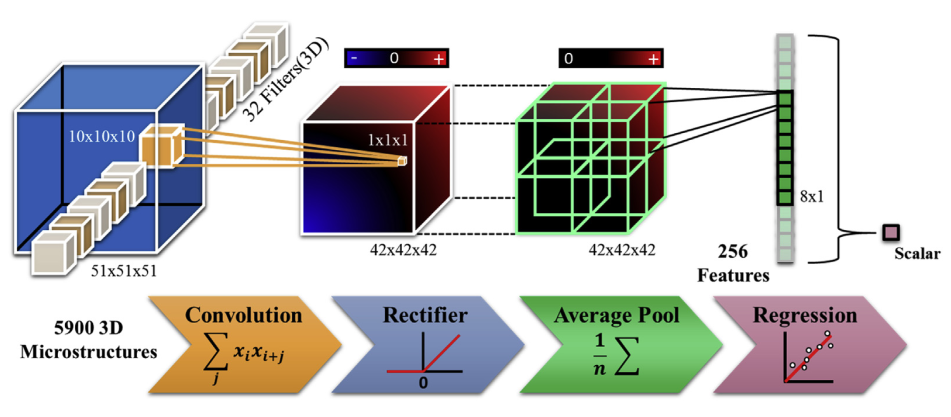
\includegraphics{pres_imgs/intro_slide.png}
\caption{image.png}
\end{figure}

\begin{itemize}
\tightlist
\item
  image: Ahmet Cecen et al., Acta Materialia 146 (2018) 76e84
\end{itemize}

    Overview

\begin{itemize}
\tightlist
\item
  Description of Neural Network Model
\item
  Training a Neural Network Model: Backpropogation
\item
  Applications of Neural Net models in materials domain
\item
  Popular Libraries : How to NN?
\item
  Convolutional Neural Networks
\item
  Analogy between CNNs and MKS Localization
\item
  PDE-NETs and learning Differential Equations using Conv-Net filters
\end{itemize}

    The inevitable brain analogy and the Perceptron

\begin{figure}
\centering
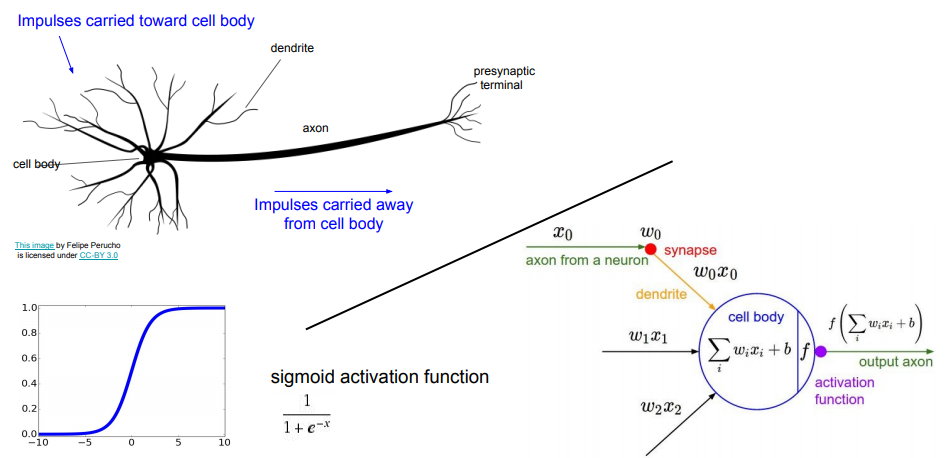
\includegraphics{pres_imgs/neuron_and_perceptron.png}
\caption{StanfordLectureNotes}
\end{figure}

    Zooming in on the Perceptron

\begin{figure}
\centering
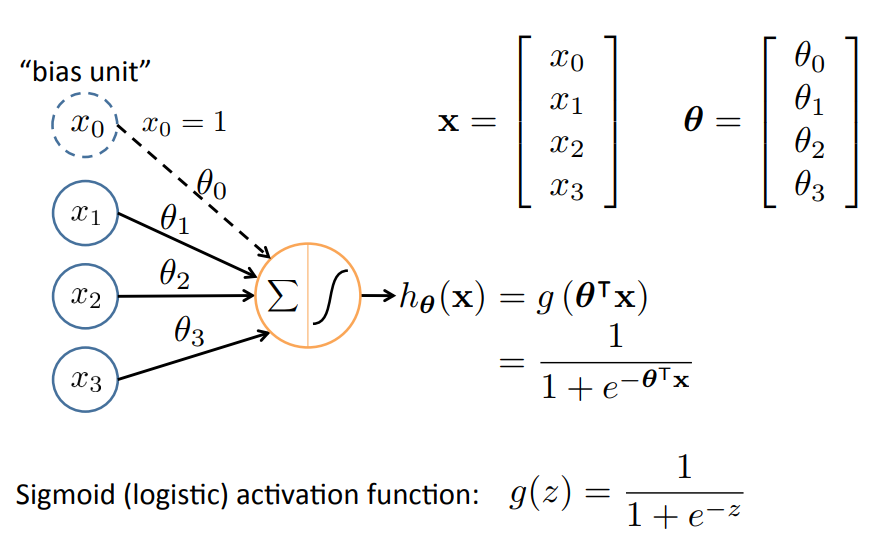
\includegraphics{pres_imgs/perceptron.png}
\caption{StanfordLectureNotes}
\end{figure}

    The neural network model

\hypertarget{a-simple-linear-model}{%
\subsection{A simple linear model}\label{a-simple-linear-model}}

\begin{itemize}
\tightlist
\item
  \(f = Wx\)

  \begin{itemize}
  \tightlist
  \item
    \(x=\{x_1, x_2,\cdots,x_n\}\)
  \item
    \$ W = \textbackslash{}begin\{pmatrix\}w\_\{11\} \& w\_\{12\} \&
    \cdots \& w\_\{1n\} \textbackslash{}w\_\{21\} \& w\_\{22\} \&
    \cdots \& w\_\{2n\} \textbackslash{} \vdots\& \vdots \& \ddots \&
    \vdots \textbackslash{} a\_\{m1\} \& w\_\{m2\} \& \cdots \&
    w\_\{mn\}\\
    \textbackslash{}end\{pmatrix\}\$
  \item
    \(f = \{f_1, f_2,\cdots,f_m\}\)
  \end{itemize}
\end{itemize}

\$ x\$ : \((n \times 1)\), \(W_1\) : \((m1 \times n)\), \(f\) :
\((m1 \times 1)\)

    The neural network model

A simple linear model * \(f = Wx\)

A 2-layer Neural Network * \(f = W_2 max(0, W_1x)\)

\$ max(0,x)\$ is known as the ReLU (Regularized Linear Unit) function

\(x\) : (\(n \times 1\)), \(W_1\) : (\(m1 \times n\)), \(W_2\) :
(\(m2 \times m1\)), \(f\) : (\(m2 \times 1\))

    The neural network model

A simple linear model * \(f = Wx\)

A 2-layer Neural Network * \(f = W_2 max(0, W_1x)\)

or A 3-layer Neural Network * \(f = W_3max(0, W_2 max(0, W_1x))\)

\(x\): (\(n \times 1\)), \(W_1\): (\(m1 \times n\)), \(W_2\):
(\(m2 \times m1\)), \(W_3\): (\(m3 \times m2\)), \(f\):
(\(m3 \times 1\))

    The neural network model

A simple linear model * \(f = Wx\)

A 2-layer Neural Network * \(f = W_2 max(0, W_1x)\)

or if you fancy, 3-layer network with both ReLU and Sigmoid activation *
\(f = W_3max(0, W_2 \sigma(W_1x))\) where
\(\sigma(h) = \dfrac{1}{1 - \exp{-h}}\)

\(x\) : (\(n \times 1\)), \(W_1\) : (\(m1 \times n\)), \(W_2\) :
(\(m2 \times m1\)), \(W_3\) : (\(m3 \times m2\)), \(f\) :
(\(m3 \times 1\))

    Commonly Used Activation Functions

\begin{figure}
\centering
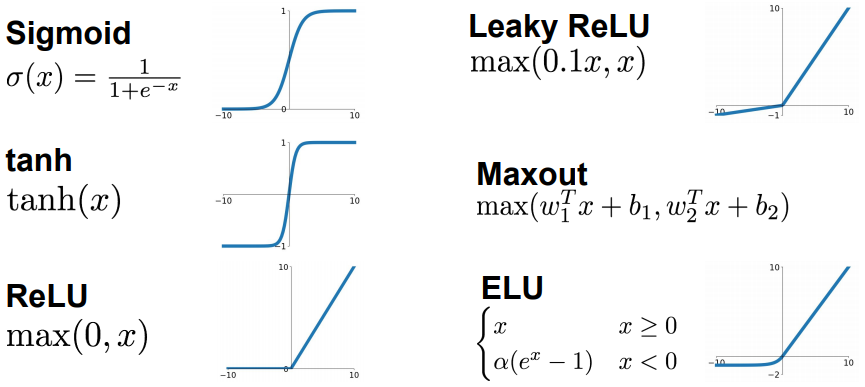
\includegraphics{pres_imgs/activation_functions.png}
\caption{StanfordLectureNotes}
\end{figure}

\begin{itemize}
\tightlist
\item
  Sigmoid and tanh functions is most commonly used in MultiLayer
  Perceptron models, whereas ReLU is the standard for conv-nets
  described later.
\item
  Please note that the derivatives of all these functions are really
  easy to compute, for eg:
  \(\dfrac{d \sigma(x)}{d(x)} = \sigma(x)(1-\sigma(x))\)
\end{itemize}

    The Neural Network as a Computational Graph

\begin{figure}
\centering
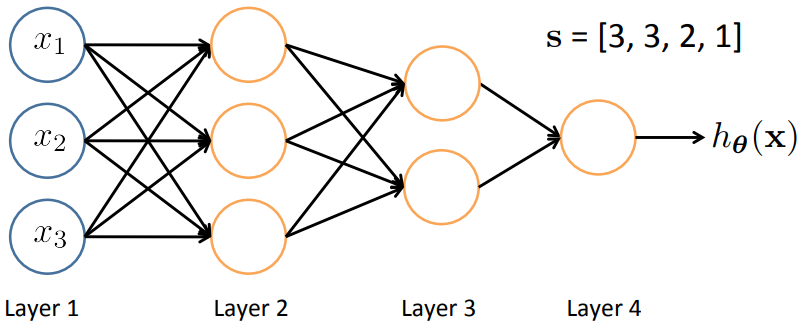
\includegraphics{pres_imgs/graph_representation.png}
\caption{StanfordLectureNotes}
\end{figure}

\begin{itemize}
\tightlist
\item
  s denotes the number of nodes(perceptrons) in each layer
\item
  This is a fully connected multi-layered perceptron model
\item
  Implemented in scikit-learn as the MLPC model and also available in
  the MATLAB machine learning toolbox
\end{itemize}

    Training the model: Optimizing the loss function

Consider the linear regression model: - \(y = w^Tx\)

    Training the model: Optimizing the loss function

Consider the linear model: - \(y = w^Tx\)

We can define a function \(\mathcal{L}\): \begin{align}
    \mathcal{L(w)} &= \sum^{N}(\hat{y_i} - y_i)^2\\
    &= \sum^{N}(\hat{y_i} - w^Tx_i)^2
\end{align} such that the problem of guessing the weights reduces to the
problem of minimizing the function \(\mathcal{L}\) also known as the
loss function.

    Training the model: Optimizing the loss function

Consider the linear model: - \(y = w^Tx\)

We can define a function \(\mathcal{L}\): \begin{align}
    \mathcal{L(w)} &= \sum^{N}(\hat{y_i} - y_i)^2\\
    &= \sum^{N}(\hat{y_i} - w^Tx_i)^2
\end{align} such that the problem of guessing the weights reduces to the
problem of minimizing the function \(\mathcal{L}\) also known as the
loss function.

\textbf{In this case, the function \(\mathcal{L}\) is clearly convex,
i.e.~a parabola in \(w\) space, so we have an analytical solution to the
problem as:} - \(\hat{w} = (X^TX)^{-1}X^T\hat{Y}\) where \(X: \{x_i\}\)
and \(\hat{Y}: \{\hat{y}_i\}\)

    Training the model: Gradient Descent

\begin{figure}
\centering
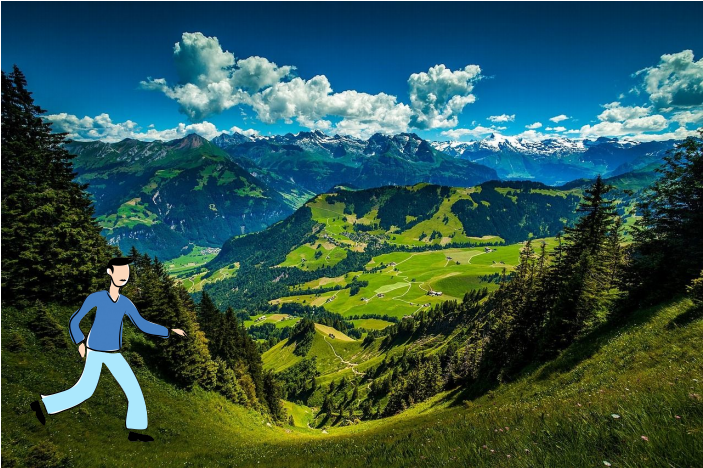
\includegraphics{pres_imgs/mountains.png}
\caption{StanfordLectureNotes}
\end{figure}

    Training the model: Gradient Descent

\begin{itemize}
\item
  The gradient at any point in the loss function denoted as
  \emph{\(\nabla_w\mathcal{L}\)}
\item
  It is a vector that gives the direction of maximal positive change in
  the loss function.
\item
  As such, loss function can be minimized by moving in the direction
  opposite to the gradient.
\item
  This gives us an update rule

  \begin{itemize}
  \tightlist
  \item
    \(w_{i}^{t+1} = w_{i}^{t} - \lambda \dfrac{\partial \mathcal{L(w)}}{\partial{w_i}}\)
  \item
    \(\lambda\) is reffered to as the learning rate and controls the
    speed of descent.
  \end{itemize}
\end{itemize}

    \begin{figure}
\centering
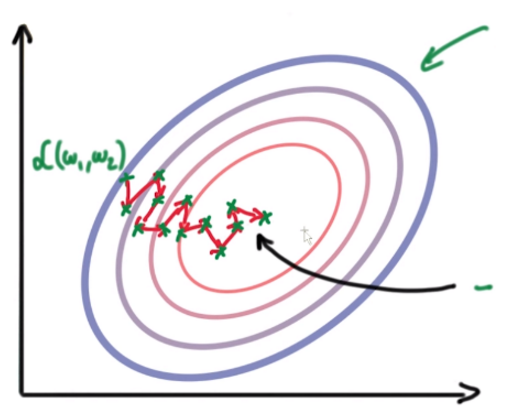
\includegraphics{pres_imgs/grad_descent.png}
\caption{StanfordLectureNotes}
\end{figure}

    Training the model: Stochastic Gradient Descent

\begin{itemize}
\tightlist
\item
  Recal:

  \begin{itemize}
  \tightlist
  \item
    \(\mathcal{L} = \dfrac{1}{N}\sum^{N}(\hat{y}_i - f(x_i))^{2}\)
  \end{itemize}
\item
  For large datasets, it is expensive to compute loss for the entire
  dataset in each update step.
\item
  An alternative is to compute gradient over batches of training data.
\item
  \textbf{Stochastic refers to the fact that the ``mini-batch'' loss
  function is a ``stochastic'' approximation of the actual loss}
\item
  This gives us a modified update rule

  \begin{itemize}
  \tightlist
  \item
    \(w_{i}^{t+1} = w_{i}^{t} - \lambda \dfrac{\partial \mathcal{l_j(w)}}{\partial{w_i}}\)
  \item
    \(\lambda\) is reffered to as the learning rate and controls the
    speed of descent.
  \end{itemize}
\end{itemize}

    Training the model: Backpropogation

\begin{itemize}
\tightlist
\item
  Recal the form of the 3-layer Neural Network Model:

  \begin{itemize}
  \tightlist
  \item
    \(f = W_3max(0, W_2 max(0, W_1x))\)
  \end{itemize}
\end{itemize}

    Training the model: Backpropogation

\begin{itemize}
\tightlist
\item
  Recal the form of the 3-layer Neural Network Model:

  \begin{itemize}
  \tightlist
  \item
    \(f = W_3max(0, W_2 max(0, W_1x))\)
  \end{itemize}
\item
  We again define the loss function as:

  \begin{itemize}
  \tightlist
  \item
    \(\mathcal{L} = \dfrac{1}{N}\sum^{N}(\hat{y}_i - f(x_i))^{2}\)
  \end{itemize}
\end{itemize}

    Training the model: Backpropogation

\begin{itemize}
\tightlist
\item
  Recal the form of the 3-layer Neural Network Model:

  \begin{itemize}
  \tightlist
  \item
    \(f = W_3\sigma(W_2 \sigma(W_1x))\)
  \end{itemize}
\item
  We again define the loss function as:

  \begin{itemize}
  \tightlist
  \item
    \(\mathcal{L} = \dfrac{1}{N}\sum^{N}(\hat{y}_i - f(x_i))^{2}\)
  \end{itemize}
\item
  We would like to use the gradient descent strategy for optimizing
  \(L\) which is:

  \begin{itemize}
  \tightlist
  \item
    \(w_{i,j}^{l}[t+1] = w_{i,j}^{l}[t] - \lambda \dfrac{\partial \mathcal{L(w[t])}}{\partial{w^l_{i,j}[t]}}\)
  \item
    where l is the index of the layer and i,j are indices of the
    parameter in the parameter matrix
  \end{itemize}
\item
  However, because of the deep nesting of weights, it is difficult to
  the get the analytic form of the partial derivative:

  \begin{itemize}
  \tightlist
  \item
    \(\dfrac{\partial \mathcal{L(w[t])}}{\partial{w^l_{i,j}[t]}}\)
  \end{itemize}
\end{itemize}

    Training the model: Backpropogation

\hypertarget{what-if-we-use-chain-rule}{%
\subsection{What if we use chain
rule?}\label{what-if-we-use-chain-rule}}

Recall, chain rule:\\
\begin{align}
\dfrac{d(f\cdot g)(x)}{dx} = \dfrac{f(g(x))}{d(g(x))}\dfrac{d(g(x))}{dx}
\end{align}

\begin{itemize}
\tightlist
\item
  A simplified illustration of backpropogation using the univariate
  logistic least squares model
\end{itemize}

\begin{figure}
\centering
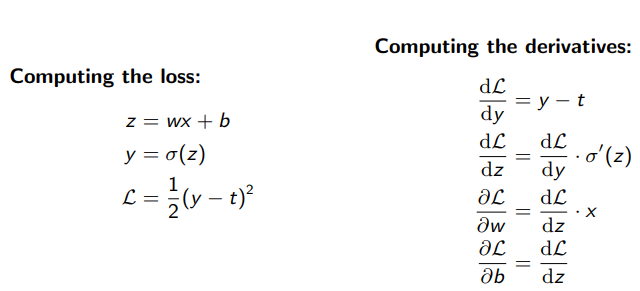
\includegraphics{pres_imgs/back_prop_simple.png}
\caption{StanfordLectureNotes}
\end{figure}

http://www.cs.toronto.edu/\textasciitilde{}rgrosse/courses/csc321\_2017/slides/lec6.pdf

    Training the model: Backpropogation

\begin{figure}
\centering
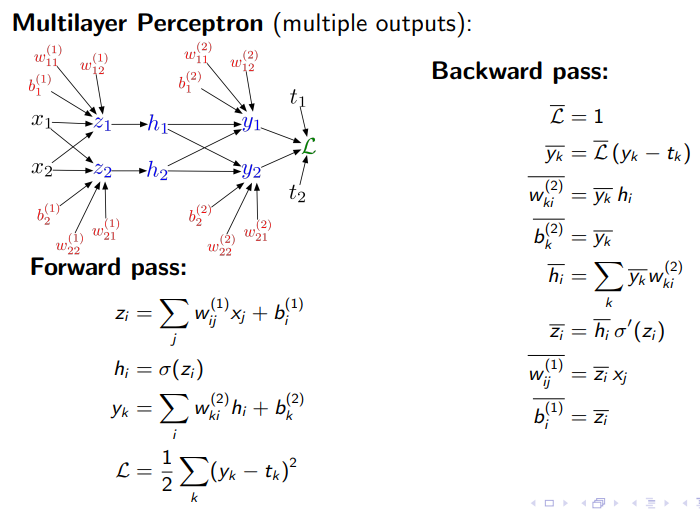
\includegraphics{pres_imgs/back_prop_mlpc.png}
\caption{StanfordLectureNotes}
\end{figure}

    Training the model: Backpropogation

\begin{figure}
\centering
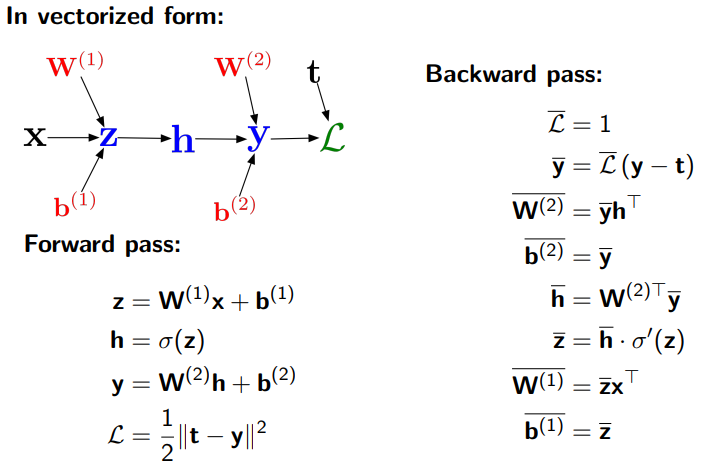
\includegraphics{pres_imgs/back_prop_mlpc_vectorized.png}
\caption{StanfordLectureNotes}
\end{figure}

    Training the model: Backpropogation

\begin{itemize}
\tightlist
\item
  In the message passing notation:
\end{itemize}

\begin{figure}
\centering
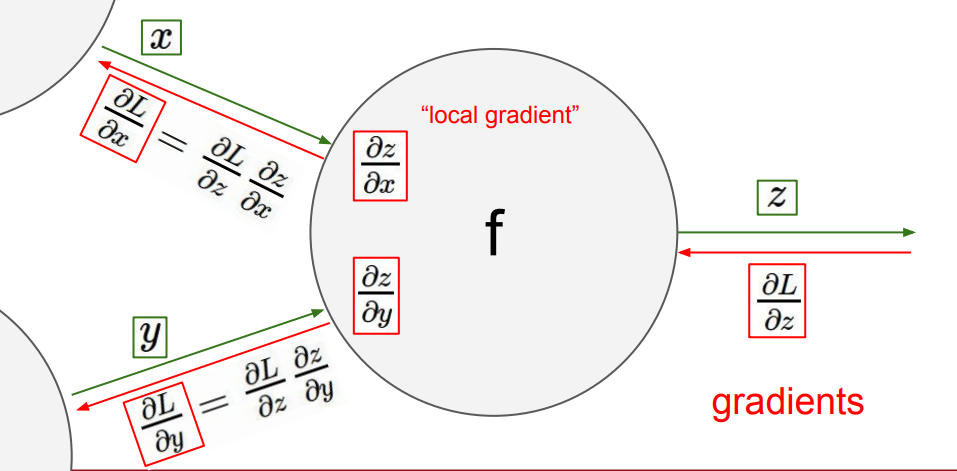
\includegraphics{pres_imgs/back-prop.png}
\caption{StanfordLectureNotes}
\end{figure}

\begin{itemize}
\tightlist
\item
  For each training step, a forward pass results in the computation of
  the loss value
\item
  A backward pass results in the updation of the weigts
\end{itemize}

    Back to the equation

\hypertarget{a-3-layer-feed-forward-neural-network}{%
\subsubsection{A 3-layer feed-forward Neural
Network}\label{a-3-layer-feed-forward-neural-network}}

\begin{itemize}
\tightlist
\item
  \(f = W_3max(0, W_2 max(0, W_1x))\)
\end{itemize}

\hypertarget{to-summarize}{%
\subsubsection{To Summarize:}\label{to-summarize}}

\begin{itemize}
\tightlist
\item
  A multilayered perceptron is a just a set of linear followed by
  non-linear transforms performed on a input vector.
\item
  A feed-forward fully connected neural network with a single hidden
  layer using practically any nonlinear activation function can
  approximate any continuous function of any number of real variables on
  any compact set to any desired degree of accuracy.
\item
  Number of Parameters in the model = \(\sum_{i=1}^{N} (L_{n-1}+1)*L_n\)
\item
  \textbf{How to guess the values of these parameters?}
\item
  https://papers.nips.cc/paper/874-how-to-choose-an-activation-function.pdf
\end{itemize}

    Resources for implementing Neural Networks

\begin{itemize}
\tightlist
\item
  Pytorch - http://pytorch.org/
\item
  Tensorflow - http://tensorflow.org/
\item
  Theano - http://deeplearning.net/software/theano/
\item
  Keras - https://keras.io/
\end{itemize}

A useful learning resource - https://playground.tensorflow.org/

Background http://cs231n.github.io/

    Convolutional Neural Networks

\begin{figure}
\centering
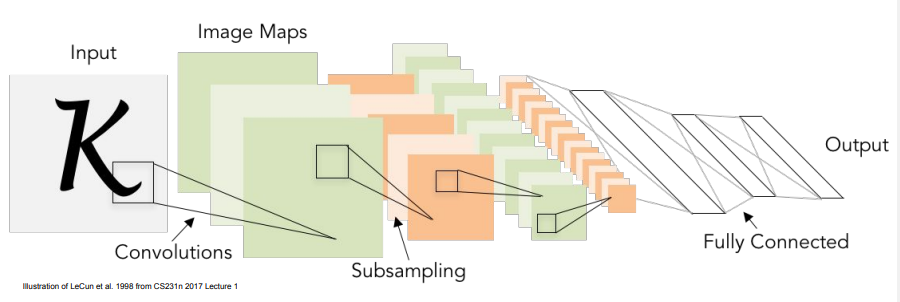
\includegraphics{pres_imgs/CNN_template.png}
\caption{StanfordLectureNotes}
\end{figure}

Gradient Based Learning applied to document recognition {[}LeCun,
Bottou, Bengio, Haffner 1998{]}

    Convolutional Neural Networks

\begin{itemize}
\item
  Image data are high dimensional and have local embedded structures.
\item
  CNNs were conceptualized to overcome the limitations of Fully
  Connected neural networks in processing image data
\end{itemize}

    Convolutional Neural Networks

\begin{figure}
\centering
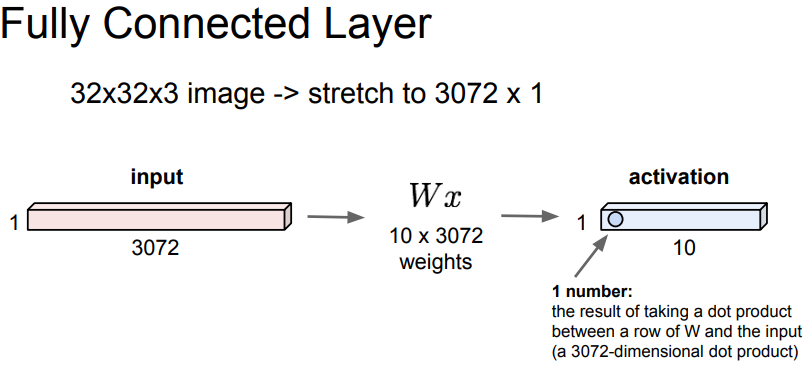
\includegraphics{pres_imgs/fc_layer.png}
\caption{StanfordLectureNotes}
\end{figure}

    Convolutional Neural Networks

\begin{figure}
\centering
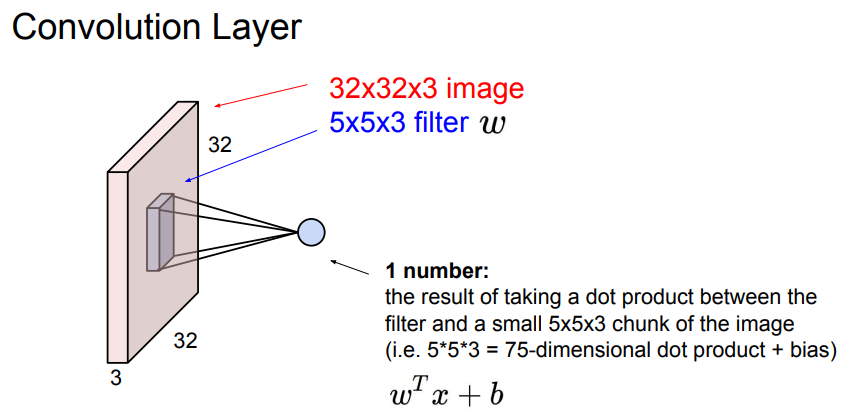
\includegraphics{pres_imgs/conv_layer_1.png}
\caption{StanfordLectureNotes}
\end{figure}

    Recall convolution:

\begin{align}
f[x, y] * g[x,y] = \sum_{n_1 = -\inf}^{\inf}\sum_{n_2 = -\inf}^{\inf} f[n_1, n_2]\cdot g[x-n_1, y-n_2]
\end{align}

    Convolutional Neural Networks

\begin{figure}
\centering
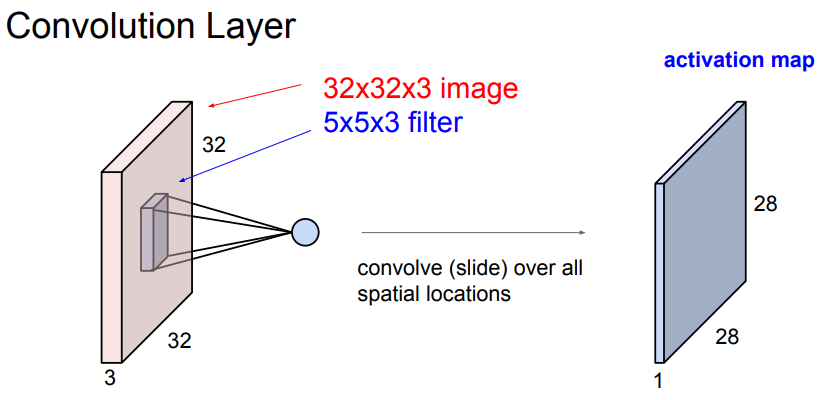
\includegraphics{pres_imgs/conv_layer_2.png}
\caption{StanfordLectureNotes}
\end{figure}

    Convolutional Neural Networks

\begin{figure}
\centering
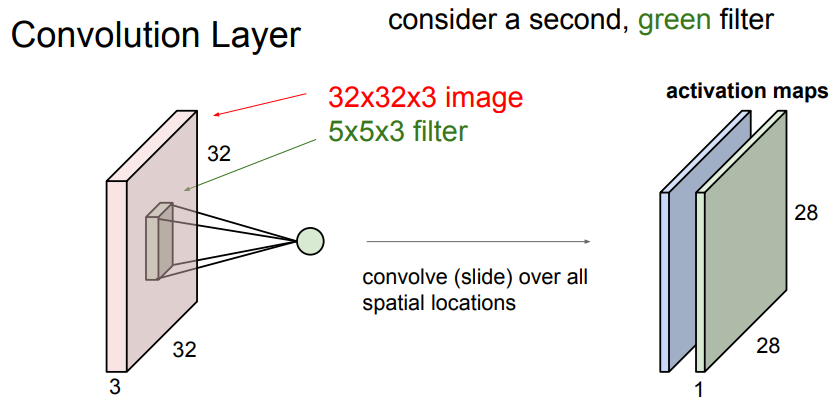
\includegraphics{pres_imgs/conv_layer_3.png}
\caption{StanfordLectureNotes}
\end{figure}

    Convolutional Neural Networks

\begin{figure}
\centering
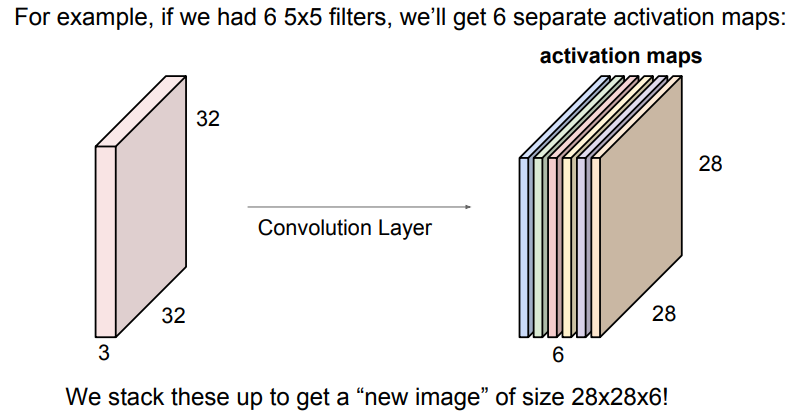
\includegraphics{pres_imgs/conv_layer_4.png}
\caption{StanfordLectureNotes}
\end{figure}

    Convolutional Neural Networks

\begin{figure}
\centering
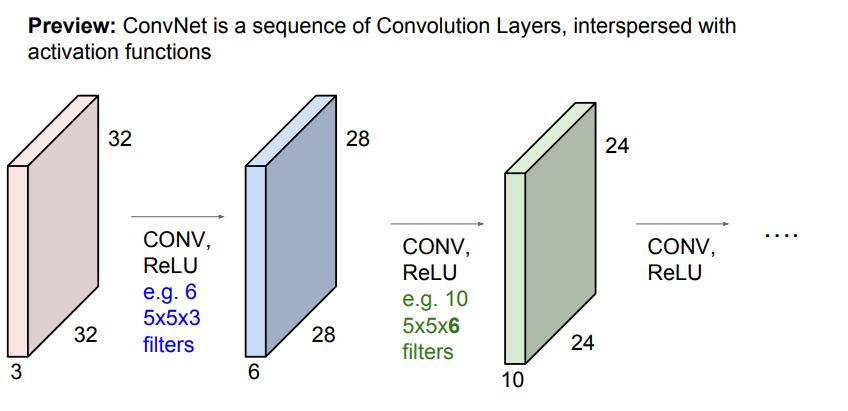
\includegraphics{pres_imgs/conv_net_full.png}
\caption{StanfordLectureNotes}
\end{figure}

    Convolutional Neural Networks

\hypertarget{inorder-to-reduce-number-of-parameters-and-prevent-overfitting.}{%
\subsection{Inorder to reduce number of parameters and prevent
overfitting.}\label{inorder-to-reduce-number-of-parameters-and-prevent-overfitting.}}

\begin{figure}
\centering
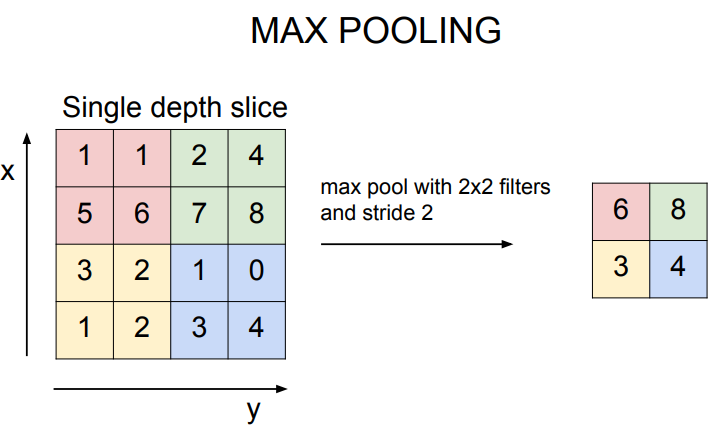
\includegraphics{pres_imgs/pooling.png}
\caption{StanfordLectureNotes}
\end{figure}

    Convolutional Neural Networks

\hypertarget{typical-off-the-shelf-cnn-deep-learning-model}{%
\subsection{Typical off the shelf CNN / Deep Learning
Model}\label{typical-off-the-shelf-cnn-deep-learning-model}}

\hypertarget{representation-learning-versus-template-learning}{%
\subsubsection{Representation Learning versus Template
learning}\label{representation-learning-versus-template-learning}}

\hypertarget{a-compaction-of-the-typical-approach-of-mks-workflow-which-involves-first-feature-generation-followed-by-linkage}{%
\subsubsection{A compaction of the typical approach of MKS workflow
which involves first feature generation followed by
linkage}\label{a-compaction-of-the-typical-approach-of-mks-workflow-which-involves-first-feature-generation-followed-by-linkage}}

\begin{figure}
\centering
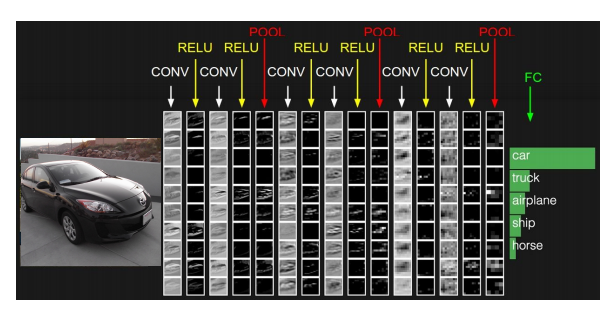
\includegraphics{pres_imgs/typical_cnn.png}
\caption{StanfordLectureNotes}
\end{figure}

    Convolutional Neural Networks

\hypertarget{vgg-net-a-production-cnn}{%
\subsection{VGG-Net : A Production CNN}\label{vgg-net-a-production-cnn}}

\begin{figure}
\centering
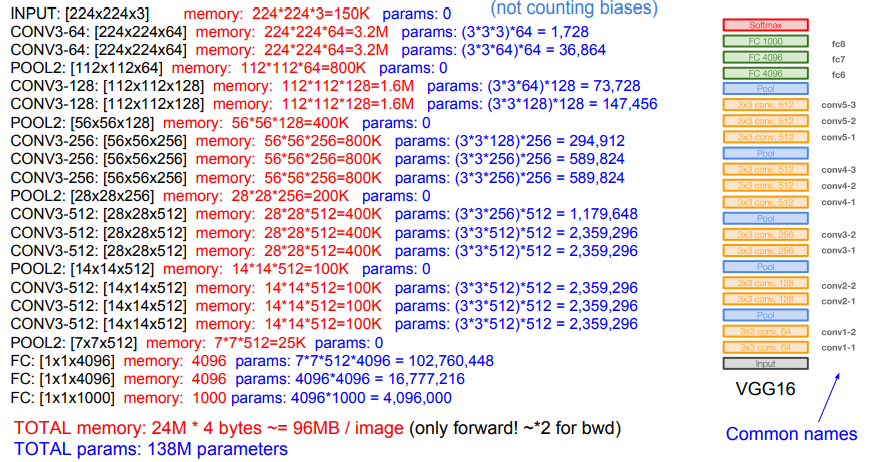
\includegraphics{pres_imgs/vgg_net.png}
\caption{StanfordLectureNotes}
\end{figure}

    Convolutional Neural Networks

\hypertarget{why-you-should-care}{%
\subsection{Why you should care?}\label{why-you-should-care}}

\begin{figure}
\centering
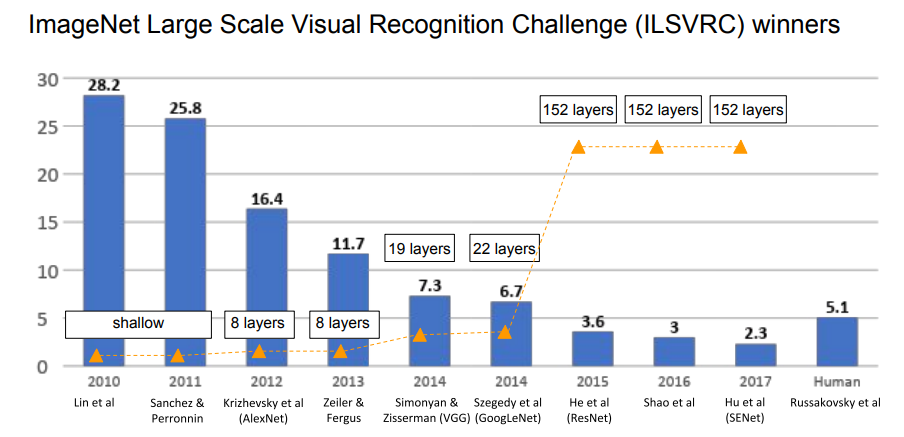
\includegraphics{pres_imgs/image_net.png}
\caption{StanfordLectureNotes}
\end{figure}


    % Add a bibliography block to the postdoc
    
    
    
    \end{document}
